\section{Position-sensitive detector}

\subsection{Transverse photoeffect}

% TODO: change variable names I_sat -> I_s etc.

The purpose of the following section is to recall the mechanics of the (transverse) photoeffect observed in an illuminated p-n junction.
Figures and the description thereof is largely based on Ref.~\cite{Simon13}.
A subtle difference in the depicted figures and the figures of Ref.~\cite{Simon13} is that we exchanged the order of p- and n-type semiconductors.
We found this order to be more intuitive when referring to a p-n junction.

\Cref{fig:pn_junction_separated} shows a separated p- and n-type semiconductor.
In the upper half, we see an illustration of the p- and n-type semiconductor with their respective mobile charge carriers.
The p-type semiconductor has an excess of positive charge carriers (holes) which are depicted as white circles.
The n-type semiconductor has an excess of negative charge carriers (electrons) which are depicted as black circles.
The excess charge carriers form due to the implantation of acceptor and donator ions.
These are depicted as circles with plus and minus sign in \Cref{fig:pn_junction_separated}.
The implanted ions have more or fewer electrons than the atoms of the semiconductor material.
Therefore donating an electron or accepting an electron and effectively forming a hole as an absence of negative charge.
\begin{figure}[H]
	\centering
	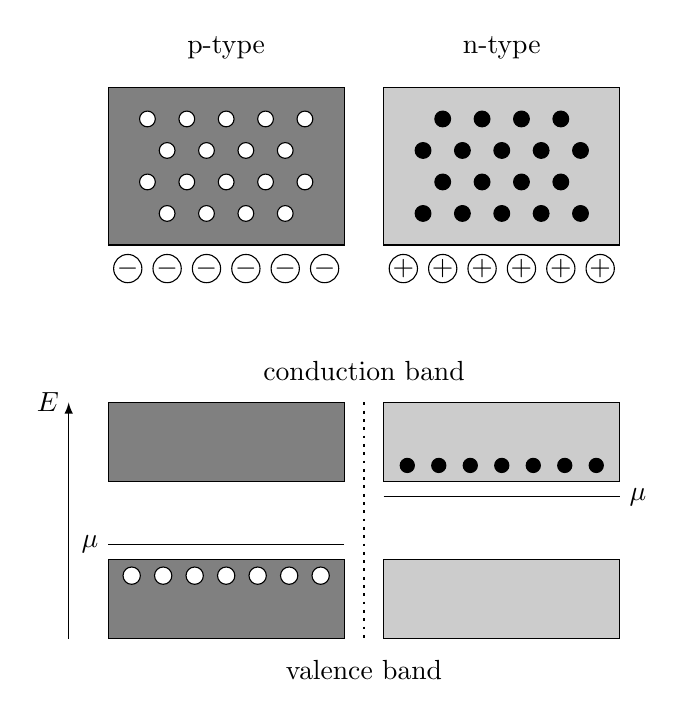
\begin{tikzpicture}
		\draw (1.5, 2.5) node {p-type};
		\draw (5, 2.5) node {n-type};
		\filldraw[draw=black, fill=gray] (0, 0) rectangle (3, 2);
		\filldraw[draw=black, fill=gray!40] (3.5, 0) rectangle (6.5, 2);
		\foreach \x in {1, ..., 4} {
			\filldraw[fill=white] (0.25+0.5*\x, 0.4) circle (.1);
			\filldraw[fill=white] (0.25+0.5*\x, 1.2) circle (.1);

			\filldraw[fill=black] (3.75+0.5*\x, 0.8) circle (.1);
			\filldraw[fill=black] (3.75+0.5*\x, 1.6) circle (.1);
		}
		\foreach \x in {1, ..., 5} {
			\filldraw[fill=white] (0.5*\x, 0.8) circle (.1);
			\filldraw[fill=white] (0.5*\x, 1.6) circle (.1);
			
			\filldraw[fill=black] (3.5+0.5*\x, 0.4) circle (.1);
			\filldraw[fill=black] (3.5+0.5*\x, 1.2) circle (.1);
		}
		\foreach \x in {0, ..., 5} {
			\draw (0.25+0.5*\x, -0.3) node[circle, draw=black, inner sep=0]{$-$};
			\draw (3.75+0.5*\x, -0.3) node[circle, draw=black, inner sep=0]{$+$};
		}
		\draw[-latex] (-0.5, -5) -- (-0.5, -2) node[left]{$E$};
		\draw[dotted, line width=1] (3.25, -2) -- (3.25, -5);
		\filldraw[draw=black, fill=gray] (0, -2) rectangle +(3, -1) +(0, -1.8) node[left]{$\mu$} -- +(3, -1.8) ++(0, -2) rectangle +(3, -1);
		\filldraw[draw=black, fill=gray!40] (3.5, -2) rectangle +(3, -1) +(0, -1.2) -- +(3, -1.2) node[right]{$\mu$} ++(0, -2) rectangle +(3, -1);
		\draw (3.25, -1.6) node{conduction band} +(0, -3.8) node{valence band};
		\foreach \x in {0, ..., 6} {
			\filldraw[fill=white] (0.3+0.4*\x, -4.2) circle (.11);
			\filldraw[fill=black] (3.8+0.4*\x, -2.8) circle (.09);
		}
	\end{tikzpicture}
	\caption{Separated p- and n-type semiconductor with holes (white) and electrons (black).}\label{fig:pn_junction_separated}
\end{figure}
The lower half of \Cref{fig:pn_junction_separated} shows the energy band structure of both p- and n-type semiconductor.
The lower energy band represents the valence band made up of the electrons that are tightly bound to a single atomic core.
The upper energy band represents the conduction band made up of electrons that are are not bound to a single atomic core but shared across the lattice.
Charge carriers in the conduction band can move freely and thereby contribute to the conductivity of the material.
For an undoped (intrinsic) semiconductor the chemical potential is in the center of the band gap between the conduction and valence band.
Through doping, the chemical potential is shifted in the p- and n-type semiconductor.
In the p-type semiconductor, acceptor ions can take up electrons from the conduction band, thereby decreasing the chemical potential.
In the n-type semiconductor, donator ions contribute electrons to the conduction band, thereby increasing the chemical potential.
\begin{figure}[H]
	\centering
	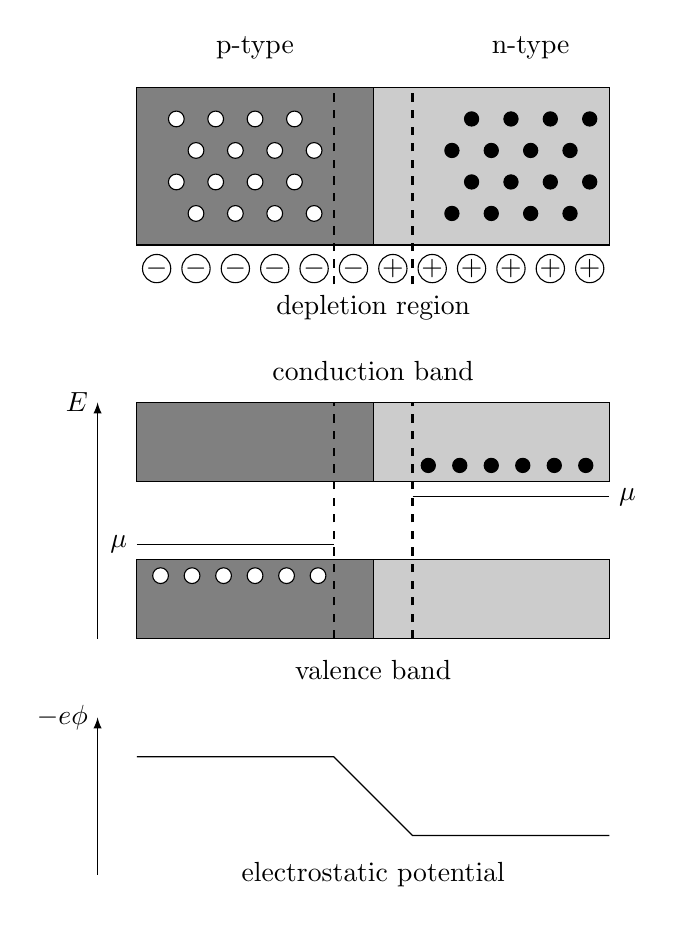
\begin{tikzpicture}
		\draw (1.5, 2.5) node {p-type};
		\draw (5, 2.5) node {n-type};
		\filldraw[draw=black, fill=gray] (0, 0) rectangle (3, 2);
		\filldraw[draw=black, fill=gray!40] (3, 0) rectangle (6, 2);
		\foreach \x in {1, ..., 4} {
			\filldraw[fill=white] (0.25+0.5*\x, 0.4) circle (.1);
			\filldraw[fill=white] (0.25+0.5*\x, 1.2) circle (.1);

			\filldraw[fill=black] (3.75+0.5*\x, 0.8) circle (.09);
			\filldraw[fill=black] (3.75+0.5*\x, 1.6) circle (.09);
		}
		\foreach \x in {1, ..., 4} {
			\filldraw[fill=white] (0.5*\x, 0.8) circle (.1);
			\filldraw[fill=white] (0.5*\x, 1.6) circle (.1);
			
			\filldraw[fill=black] (3.5+0.5*\x, 0.4) circle (.09);
			\filldraw[fill=black] (3.5+0.5*\x, 1.2) circle (.09);
		}
		\foreach \x in {0, ..., 5} {
			\draw (0.25+0.5*\x, -0.3) node[circle, draw=black, inner sep=0]{$-$};
			\draw (3.25+0.5*\x, -0.3) node[circle, draw=black, inner sep=0]{$+$};
		}
		\draw[dashed, line width=.8] (2.5, -.5) -- +(0, 2.5) +(1, 0) -- +(1, 2.5) +(0.5, -0.3) node{depletion region};

		\draw[-latex] (-0.5, -5) -- (-0.5, -2) node[left]{$E$};
		\filldraw[draw=black, fill=gray] (0, -2) rectangle +(3, -1) +(0, -1.8) node[left]{$\mu$} -- +(2.5, -1.8) ++(0, -2) rectangle +(3, -1);
		\filldraw[draw=black, fill=gray!40] (3, -2) rectangle +(3, -1) +(0.5, -1.2) -- +(3, -1.2) node[right]{$\mu$} ++(0, -2) rectangle +(3, -1);
		\draw[dashed, line width=.8] (2.5, -5) -- +(0, 3) +(1, 0) -- +(1, 3) +(0.5, -0.3);
		\draw (3, -1.6) node{conduction band} +(0, -3.8) node{valence band};
		\foreach \x in {0, ..., 5} {
			\filldraw[fill=white] (0.3+0.4*\x, -4.2) circle (.10);
			\filldraw[fill=black] (3.7+0.4*\x, -2.8) circle (.09);
		}
		
		\draw[-latex] (-0.5, -8) -- (-0.5, -6) node[left]{$-e\phi$};
		\draw (0, -6.5) -- ++(2.5, 0) -- ++(1, -1) -- ++(2.5, 0);
		\draw (3, -8) node{electrostatic potential};
	\end{tikzpicture}
	\caption{Combined p- and n-type semiconductor with holes (white) and electrons (black).}\label{fig:pn_junction_combined}
\end{figure}
In \Cref{fig:pn_junction_combined} the p- and n-type semiconductor are brought into contact with each other, forming a p-n junction.
In close proximity of the junction holes and energies recombine due to a diffusion process, leaving an electrically charged area.
The electrically charged area creates an electrostatic potential across the junction as illustrated in the lower part of \Cref{fig:pn_junction_combined}.
We refer to this area as the depletion region.
In \Cref{fig:pn_junction_combined} the depletion region expands between the dashed lines around the junction.
\begin{figure}[H]
	\centering
	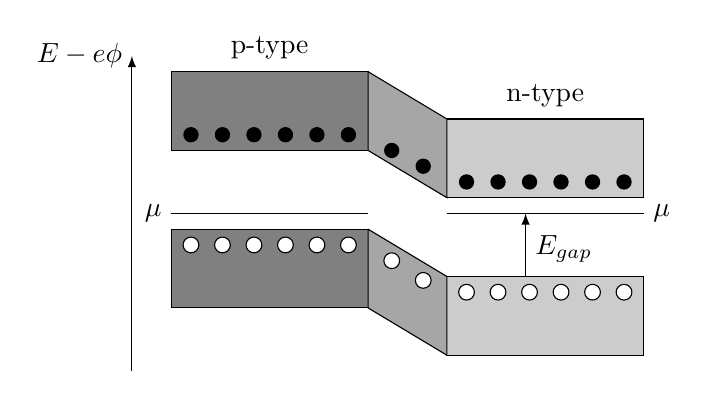
\begin{tikzpicture}
		\draw (1.25, 3.6) node {p-type};
		\draw (4.75, 3.0) node {n-type};
		\draw[-latex] (-0.5, -0.5) -- (-0.5, 3.5) node[left]{$E-e\phi$};
		\filldraw[draw=black, fill=gray] (0, 3.3) rectangle +(2.5, -1) +(0, -1.8) node[left]{$\mu$} -- +(2.5, -1.8) ++(0, -2) rectangle +(2.5, -1);
		\filldraw[draw=black, fill=gray!40] (3.5, 2.7) rectangle +(2.5, -1) +(0, -1.2) -- +(2.5, -1.2) node[right]{$\mu$} ++(0, -2) rectangle +(2.5, -1);
		\filldraw[draw=black, fill=gray!70] (2.5, 3.3) -- ++(1, -.6) -- ++(0, -1) -- ++(-1, .6) -- ++(0, 1);
		\filldraw[draw=black, fill=gray!70] (2.5, 1.3) -- ++(1, -.6) -- ++(0, -1) -- ++(-1, .6) -- ++(0, 1);
		\draw[-latex] (4.5, 0.7) -- ++(0, 0.8);
		\draw (4.5, 1.05) node[right]{$E_\text{gap}$};
		\foreach \x in {0, ..., 5} {
			\filldraw[fill=white] (0.25+0.4*\x, 1.1) circle (.10);
			\filldraw[fill=white] (3.75+0.4*\x, 0.5) circle (.10);
			\filldraw[fill=black] (3.75+0.4*\x, 1.9) circle (.09);
			\filldraw[fill=black] (0.25+0.4*\x, 2.5) circle (.09);
		};
		\filldraw[fill=white] (2.8, 0.9) circle (.10);
		\filldraw[fill=white] (3.2, 0.65) circle (.10);
		\filldraw[fill=black] (2.8, 2.3) circle (.09);
		\filldraw[fill=black] (3.2, 2.1) circle (.09);
	\end{tikzpicture}
	\caption{Energy bands of the p-n junction.}\label{fig:pn_junction}
\end{figure}
The energy band diagram in \Cref{fig:pn_junction} accounts for the shift in energy due to the electrostatic potential.
The chemical potentials of both sides of the junction are now aligned.
The energy required to excite an electron on the p-type side from the valence to the conduction band and the energy required to excite a hole from the conduction to the valence band are equal to the band gap of the semiconductor.

% TODO: motivate reverse bias (photoconductive mode) vs. unbiased (photovoltaic) mode by measurement vs. energy conversion application 
If one applies a reverse bias voltage across the p-n junction, the effective energy gap between conduction and valence band is reduced, the electrostatic potential increases and the depletion region broadens.
The situation of an applied reverse voltage is depicted in \Cref{fig:pn_junction_reverse}.
\begin{figure}[H]
	\centering
	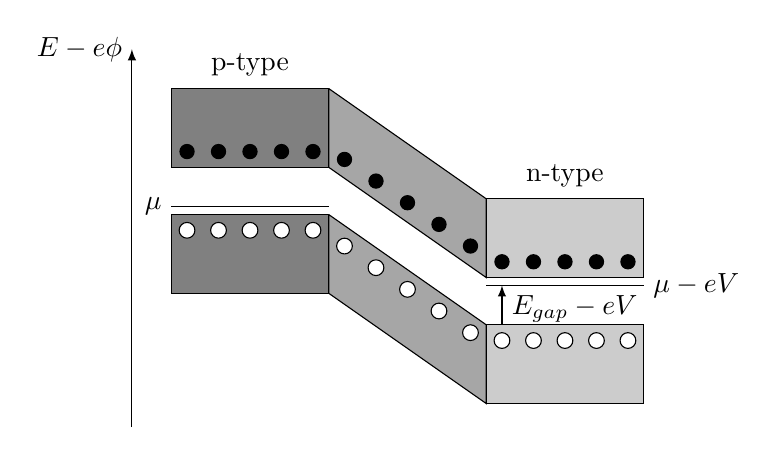
\begin{tikzpicture}
		\draw (1, 3.6) node {p-type};
		\draw (5, 2.2) node {n-type};
		\draw[-latex] (-0.5, -1) -- (-0.5, 3.8) node[left]{$E-e\phi$};
		\filldraw[draw=black, fill=gray] (0, 3.3) rectangle +(2, -1) +(0, -1.5) node[left]{$\mu$} -- +(2, -1.5) ++(0, -1.6) rectangle +(2, -1);
		\filldraw[draw=black, fill=gray!40] (4, 1.9) rectangle +(2, -1) +(0, -1.1) -- +(2, -1.1) node[right]{$\mu-eV$} ++(0, -1.6) rectangle +(2, -1);
		\filldraw[draw=black, fill=gray!70] (2, 3.3) -- ++(2, -1.4) -- ++(0, -1) -- ++(-2, 1.4) -- ++(0, 1);
		\filldraw[draw=black, fill=gray!70] (2, 1.7) -- ++(2, -1.4) -- ++(0, -1) -- ++(-2, 1.4) -- ++(0, 1);
		\draw[-latex] (4.2, 0.3) -- ++(0, 0.5);
		\draw (4.2, 0.5) node[right]{$E_\text{gap}-eV$};
		\foreach \x in {0, ..., 4} {
			\filldraw[fill=white] (0.2+0.4*\x, 1.5) circle (.10);
			\filldraw[fill=white] (2.2+0.4*\x, 1.3-0.275*\x) circle (.10);
			\filldraw[fill=white] (4.2+0.4*\x, 0.1) circle (.10);
			\filldraw[fill=black] (4.2+0.4*\x, 1.1) circle (.09);
			\filldraw[fill=black] (2.2+0.4*\x, 2.4-0.275*\x) circle (.09);
			\filldraw[fill=black] (0.2+0.4*\x, 2.5) circle (.09);
		};
	\end{tikzpicture}
	\caption{Energy band diagram of a reverse biased p-n junction.}\label{fig:pn_junction_reverse}
\end{figure}
The current-voltage characteristic of the p-n junction is described by the Schockley diode equation,
\begin{equation}
	I_\text{diode}=I_\text{sat}(T)\left(e^{eV/k_BT}-1\right)
	\label{eq:diode_current},
\end{equation}
wherein $I_\text{sat}\propto e^{-E_\text{gap}/k_BT}$ is the temperature dependent reverse bias saturation current and $V$ the voltage applied to the p-n junction.
Using the proportionality of the reverse bias saturation current, we can write,
\begin{equation}
	I_\text{diode}\propto e^{\left(eV-E_\text{gap}\right)/k_BT}-e^{-E_\text{gap}/k_BT}\label{eq:diode_current_prop},
\end{equation} 
which discloses the two effects contributing to the diode current.
The left-hand side of the proportionality of \Cref{eq:diode_current_prop} represents the current contribution due intra-band excitation of charge carriers, whereas the right-hand side represents the current contribution due to inter-band excitation.
\begin{figure}[H]
	\centering
	\begin{tikzpicture}
		\begin{axis}[xmin=-5, xmax=5, xticklabels=\empty, xlabel=$V$, ymin=-5, ymax=5, ylabel=$I$, yticklabels=\empty, axis lines=middle]
			\addplot[domain=-5:2, samples=100]{exp(x)-1-1/(x+5.4)^6};
			\addplot[domain=-5:2, samples=100]{exp(x)-1-1/(x+5.4)^6-0.5};
			\addplot[domain=-5:2, samples=100]{exp(x)-1-1/(x+5.4)^6-1};
		\end{axis}
		\draw (-0.2, 2.3) node[left]{$I_\text{sat}$} -- +(1.4, 0);
		\draw (-0.2, 1.72) node[left]{$I_\text{sat}-I_\text{photo}$} -- +(1.3, 0);
	\end{tikzpicture}
	\caption{Current-voltage characteristics of a p-n junction with different levels of illumination.}\label{fig:pn_junction_iv}
\end{figure}
In \Cref{fig:pn_junction_iv} we see the current-voltage characteristics of the p-n junction under different levels of illumination.
For negative voltages, the p-n junction is operated under reverse bias.
If the reverse bias voltage exceeds the breakdown voltage the p-n junction starts to conduct.
The current before the breakdown occurs is the reverse saturation current.
For different levels of illumination, the curve is shifted downwards.
The separation between the non-illuminated (top curve) and illuminated curves represent the respective photocurrent.
% TODO: mention non-linearity of voltage response to illumination

The conversion rate of photons to photoelectrons depends on the type of the band gap, i.e. direct or indirect, the wavelength $\lambda$ of the photon and the temperature $T$.
Most photodiodes report a wavelength $\lambda$ dependent responsitivity $R$ which can be used to convert the radiant flux $P$ of the incident light to the generated photocurrent $I_\text{photo}$,
\begin{equation}
	I_\text{photo}=RP
	\label{eq:responsitivity}.
\end{equation}
For silicon-based p-n junctions, the responsitivity $R$ is between \SI{0.2}{\ampere\per\watt} at \SI{400}{\nano\meter} and \SI{0.6}{\ampere\per\watt} at \SI{950}{\nano\meter}.

\begin{figure}[H]
	\centering
	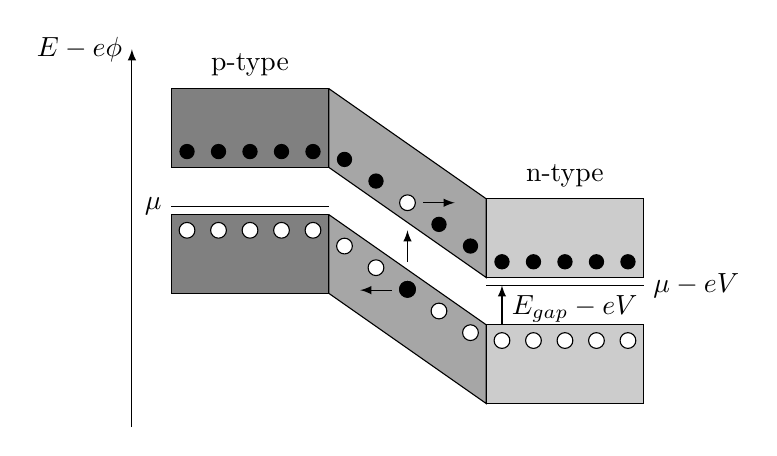
\begin{tikzpicture}
		\draw (1, 3.6) node {p-type};
		\draw (5, 2.2) node {n-type};
		\draw[-latex] (-0.5, -1) -- (-0.5, 3.8) node[left]{$E-e\phi$};
		\filldraw[draw=black, fill=gray] (0, 3.3) rectangle +(2, -1) +(0, -1.5) node[left]{$\mu$} -- +(2, -1.5) ++(0, -1.6) rectangle +(2, -1);
		\filldraw[draw=black, fill=gray!40] (4, 1.9) rectangle +(2, -1) +(0, -1.1) -- +(2, -1.1) node[right]{$\mu-eV$} ++(0, -1.6) rectangle +(2, -1);
		\filldraw[draw=black, fill=gray!70] (2, 3.3) -- ++(2, -1.4) -- ++(0, -1) -- ++(-2, 1.4) -- ++(0, 1);
		\filldraw[draw=black, fill=gray!70] (2, 1.7) -- ++(2, -1.4) -- ++(0, -1) -- ++(-2, 1.4) -- ++(0, 1);
		\draw[-latex] (4.2, 0.3) -- ++(0, 0.5);
		\draw (4.2, 0.5) node[right]{$E_\text{gap}-eV$};
		\foreach \x in {0, ..., 4} {
			\filldraw[fill=white] (0.2+0.4*\x, 1.5) circle (.10);
			\filldraw[fill=white] (2.2+0.4*\x, 1.3-0.275*\x) circle (.10);
			\filldraw[fill=white] (4.2+0.4*\x, 0.1) circle (.10);
			\filldraw[fill=black] (4.2+0.4*\x, 1.1) circle (.09);
			\filldraw[fill=black] (2.2+0.4*\x, 2.4-0.275*\x) circle (.09);
			\filldraw[fill=black] (0.2+0.4*\x, 2.5) circle (.09);
		};
		\filldraw[fill=white] (3.0, 1.85) circle (.10);
		\filldraw[fill=black] (3.0, 0.75) circle (.10);
		\draw[-latex] (3.0, 1.1) -- +(0, 0.4);
		\draw[-latex] (3.2, 1.85) -- +(0.4, 0);
		\draw[-latex] (2.8, 0.74) -- +(-0.4, 0);
	\end{tikzpicture}
	\caption{Energy diagram of a reverse biased p-n junction under illumination.}\label{fig:pn_junction_illumination}
\end{figure}
\Cref{fig:pn_junction_illumination} shows a p-n junction under reverse bias where a photon excites an electron-hole pair in the depletion region.
Due to the electrostatic potential, the electron is accelerated to the right side.
Analogue the hole is accelerated to the left side and in addition to the diode current, \Cref{eq:diode_current}, a photocurrent can be measured across the junction.

\subsection{Lateral photoeffect}

% TODO: history: lateral photoeffect Schottky30, Wallmark57

The lateral photoeffect was first discovered by W. Schottky in 1930~\cite{Schottky30}.
In 1957, it was rediscovered by J. Wallmark~\cite{Wallmark57}.

% TODO: cite Noolang and Woltring as main sources

\begin{figure}[H]
	\centering
	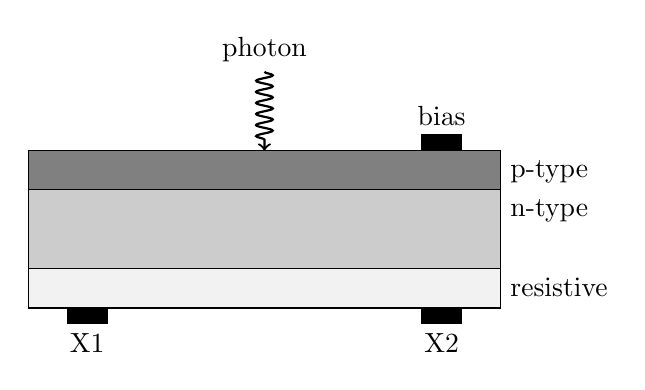
\begin{tikzpicture}
		\filldraw[fill=gray] (0, 1.5) rectangle +(6, 0.5) node[below right]{p-type};
		\filldraw[fill=gray!40] (0, 0.5) rectangle +(6, 1) node[below right]{n-type};
		\filldraw[fill=gray!10] (0, 0) rectangle +(6, 0.5) node[below right]{resistive};
		\filldraw[fill=black] (5, 2) rectangle ++(0.5, 0.2) +(-0.25, 0) node[above]{bias};
		\draw [->, thick, decorate, decoration={snake, amplitude=3, segment length=4, post length=3}] (3, 3) node[above]{photon} -- +(0, -1);
		\filldraw[fill=black] (0.5, 0) rectangle ++(0.5, -0.2) +(-0.25, 0) node[below]{X1};
		\filldraw[fill=black] (5, 0) rectangle ++(0.5, -0.2) +(-0.25, 0) node[below]{X2};
	\end{tikzpicture}
	\caption{Cross section of a lateral photodiode.}
\end{figure}

% TODO: rename rho_d -> rho and w_d -> w

% TODO: Lucovsky equations with idea (Woltring75)
\begin{equation}
	\nabla^2V=\frac{\rho}{w}J_s\left(e^{eV/k_BT}-1\right)-\frac{\rho_d}{w}J_p\label{eq:lucovsky_exact}
\end{equation}

% TODO: mention benefits of reverse bias (refer to highlighted parts in Woltring75)
\begin{align}
	\nabla^2V\approx-\frac{\rho}{w}\left(J_s+J_p\right) && \text{when } eV/k_BT\ll1 \label{eq:lucovsky_reverse_bias}	
\end{align}

\begin{equation}
	\nabla^2V_p=-\frac{\rho_d}{w_d}J_p\label{eq:lucovsky_simplified}	
\end{equation}


\begin{equation}
	V_p(x,y, t=0)=I_p\frac{\rho}{w}\delta(x-x^*)\delta(y-y^*)
	\label{eq:lucovsky_initial}	
\end{equation}

\begin{figure}[H]
	\centering
	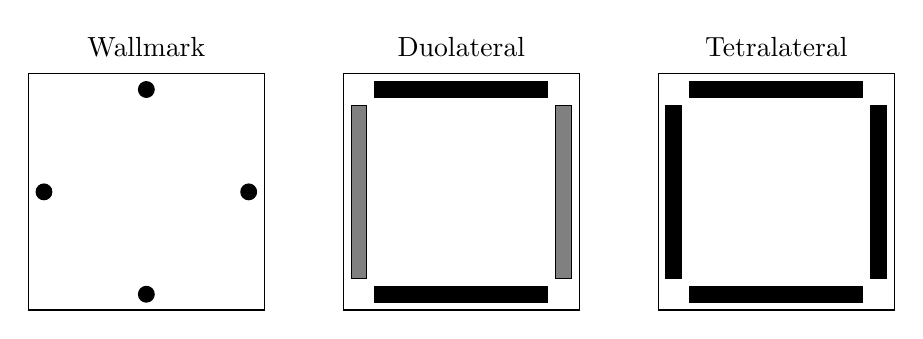
\begin{tikzpicture}
		\filldraw[fill=white] (0, 0) rectangle +(3, 3);
		\filldraw[fill=white] (4, 0) rectangle +(3, 3);
		\filldraw[fill=white] (8, 0) rectangle +(3, 3);
		\filldraw (1.5, 0.2) circle (.1);
		\filldraw (1.5, 2.8) circle (.1);
		\filldraw (0.2, 1.5) circle (.1);
		\filldraw (2.8, 1.5) circle (.1);
		\filldraw (4.4, 0.1) rectangle (6.6, 0.3);
		\filldraw (4.4, 2.7) rectangle (6.6, 2.9);
		\filldraw[fill=black!50] (4.1, 0.4) rectangle (4.3, 2.6);
		\filldraw[fill=black!50] (6.7, 0.4) rectangle (6.9, 2.6);
		\filldraw (8.4, 0.1) rectangle (10.6, 0.3);
		\filldraw (8.4, 2.7) rectangle (10.6, 2.9);
		\filldraw (8.1, 0.4) rectangle (8.3, 2.6);
		\filldraw (10.7, 0.4) rectangle (10.9, 2.6);
		\draw (1.5, 3.1) node[above]{Wallmark};
		\draw (5.5, 3.1) node[above]{Duolateral};
		\draw (9.5, 3.1) node[above]{Tetralateral};
	\end{tikzpicture}
	\caption{Contact configurations of a lateral photodiode.}
\end{figure}

% TODO: Dirichlet, Neumann boundary condition

\begin{equation}
	V^*_{nm}(x,y)=\frac{\sin(m\pi x/l)\sin(n\pi y/l)}{(m^2+n^2)\pi^2}l^2
	\label{eq:lucovsky_fourier}	
\end{equation}


\begin{equation}
	V^*_p(x,y)=I_p\frac{\rho}{w}\sum_{n\in\mathbb{Z}}\sum_{m\in\mathbb{Z}}\frac{\sin(m\pi x/l)\sin(m\pi x^*/l)\sin(n\pi y/l)\sin(n\pi y^*/l)}{(m^2+n^2)\pi^2}
	\label{eq:lucovsky_solution}
\end{equation}


% TODO: derive output current for tetralateral type
\begin{equation}
	I_{x1}(x^*,y^*)=\frac{w}{\rho}\int_0^l\dd{y}\eval{\pdv{V}{x}}_{x=0}
\end{equation}

\begin{equation}
	I_{x1}(x^*,y^*)=\frac{2}{\pi}I_p\sum_{n\in\mathbb{Z}}\frac{\sin[(2n-1)\pi y^*/l]}{2n-1}\frac{\sinh[\abs{2n-1}\pi(1-x^*/l)]}{\sinh(\abs{2n-1}\pi)}	
\end{equation}
% TODO: derive linear relation between currents and light spot position

\begin{align}
	I_{x1}(x^*,l/2)
	&=\frac{2}{\pi}I_p\sum_{n\in\mathbb{Z}}\frac{(-1)^{n+1}}{2n-1}\frac{\sinh(\abs{2n-1}\pi(1-x^*/l))}{\sinh(\abs{2n-1}\pi)}\\
	&\approx I_p\left\{0.25-0.41731\left(\frac{x}{2l}-1\right)\right\}+\mathcal{O}\left(\left(\frac{x^*}{l}-\frac{1}{2}\right)^2\right)
\end{align}


\begin{equation}
	\frac{I_{x2}(x^*,l/2)-I_{x1}(x^*,l/2)}{I_{x1}(x^*,l/2)+I_{x2}(x^*,l/2)}
	\propto\frac{x}{l}
\end{equation}


% TODO: mention benefits of tetralateral type manufacturing
% TODO: mention improved tetralateral designs (Doke87, Wang89)

\begin{align}
	\frac{\left(I_{x2}+I_{y1}\right)-\left(I_{x1}+I_{y2}\right)}{I_{x1}+I_{x2}+I_{y1}+I_{y2}}=\frac{2x}{l} &&
	\frac{\left(I_{x2}+I_{y2}\right)-\left(I_{x1}+I_{y1}\right)}{I_{x1}+I_{x2}+I_{y1}+I_{y2}}=\frac{2y}{l}	
\end{align}


\subsection{Characteristics}

% TODO: bandwidth limit
% TODO: equivalent circuit with capacitance, resistance

\begin{figure}[H]
	\centering
	\begin{circuitikz}
		\draw (0, 0) node[circ]{};
		\draw (+2, +2) node[ocirc, label=X1]{} to[photodiode] (0, 0);
		\draw (-2, -2) node[ocirc, label=X2]{} to[photodiode] (0, 0);
		\draw (+2, -2) node[ocirc, label=Y2]{} to[photodiode] (0, 0);
		\draw (-2, +2) node[ocirc, label=Y1]{} to[photodiode] (0, 0);
		\draw (0, 0) -- ++(0, -2.5) node[ocirc, label=Cathode, rotate=180]{};
	\end{circuitikz}
	\caption{Position-sensitive detector as photodiodes}
\end{figure}

\begin{figure}[H]
	% TODO: add position dependent potentiometers to anode (Andersson08 Fig. 15) 
	\centering
	\begin{circuitikz}
		\draw (-3, -2) to[current source, l=$I_\text{photo}$] ++(0, 4);
		\draw (-1, -2) node[circ]{} to[current source, l=$I_\text{dark}$] ++(0, 4) node[circ]{};
		\draw (1, -2) node[circ]{} to[resistor, l=$R_d$] ++(0, 4) node[circ]{};
		\draw (3, -2) to[capacitor, l=$C_d$] ++(0, 4);
		\draw (-3, -2) -- ++(6, 0);
		\draw (-3, 2) -- ++(6, 0);
		\draw (0, -2) -- ++(0, -1) node[ocirc, label=Cathode, rotate=180]{};
		\draw (0, 2) -- ++(0, 1) node[ocirc, label=Anode]{};
	\end{circuitikz}
	\caption{Photodiode equivalent circuit}
\end{figure}

\subsection{Noise and non-linear error}

% TODO: define signal-to-noise ratio

% TODO: photon shot noise
% TODO: thermal noise through psd resistance
% TODO: noise through leakage current and non-linearity
% TODO: non-linear errors (requires additional research)